\section{The tangent obstruction}\label{sec:tangent}

We finish the proof by taking a first-order limit in the norm identity
at a point where the kernel projection varies smoothly. This produces
a bilinear matrix whose entries must vanish by Lemma~\ref{lem:form}.

\begin{proof}[Proof of Theorem~\ref{thm:main}]
Proposition~\ref{prop:hyperbolic} establishes the polynomial's degree,
normalization, and hyperbolicity. Suppose its closed hyperbolicity cone
has a real symmetric pencil representation of some finite size.
Fix the maps \(D,E,B\) supplied by Proposition~\ref{prop:pencil}, with
their fixed finite dimensions \(a,c\). Proposition~\ref{prop:norm} gives
\eqref{eq:norm-identity} for the projections in \eqref{eq:projections}.
We shall show that this identity is impossible.

Write \(S^3=\{u\in\R^4:\norm{u}=1\}\) and consider the symmetric matrix
\[
 A(u)=E(I-uu^\top),\qquad
 u\in\Omega:=\{u\in S^3:u_0\ne0\}.
\]
Its ranks take only finitely many values, so their maximum \(\rho\) is
attained at some \(v\in\Omega\). If \(\rho>0\), select \(\rho\) independent
columns of \(A(v)\), and let \(W(u)\) contain the same columns of \(A(u)\).
These columns remain independent on a neighborhood of \(v\) in
\(\Omega\). By maximality of \(\rho\), they span the range of \(A(u)\)
throughout that neighborhood. Symmetry of \(A(u)\) then gives
\[
 R(u)=I-W(u)\bigl(W(u)^\top W(u)\bigr)^{-1}W(u)^\top .
\]
This is a smooth matrix function. If \(\rho=0\), then \(R(u)=I\) on
\(\Omega\), so it is smooth in this case as well.

Keep \(v\) fixed. At \(u=v\), Equation~\eqref{eq:norm-identity} gives
\[
 P(v)B(y)R(v)=0\qquad(y\in\R^3),
\]
because \(b(0,y)=0\). For \(h=(h_0,h')\in v^\perp\), define
\[
 Jh=v_0h'-h_0v',
 \qquad
 u_s=\frac{v+sh}{\sqrt{1+s^2\norm{h}^2}}.
\]
For small \(s\), this path stays in the neighborhood where \(R\) is
smooth, and its velocity at zero is \(h\). Moreover,
\[
 v_0u_s'-(u_s)_0v'
   =\frac{s\,Jh}{\sqrt{1+s^2\norm{h}^2}}.
\]
Thus, for \(s\ne0\), homogeneity of \(b\) and
\eqref{eq:norm-identity} give
\[
 \frac{b(Jh,y)}{1+s^2\norm{h}^2}
 =
 \norm{P(v)B(y)\frac{R(u_s)-R(v)}{s}}_{\op}^{2}.
\]
The matrix difference quotient converges to the differential
\(dR_v(h)\). Passing to the limit by continuity of the operator norm
yields
\begin{equation}\label{eq:tangent-identity}
 b(Jh,y)=\norm{P(v)B(y)dR_v(h)}_{\op}^{2}
 \qquad(h\in v^\perp,\ y\in\R^3).
\end{equation}
Only \(R\) has been differentiated; the projection \(P(v)\) remains
fixed. Figure~\ref{fig:local-tangent} illustrates this local variation.

\begin{figure}[htbp]
\centering
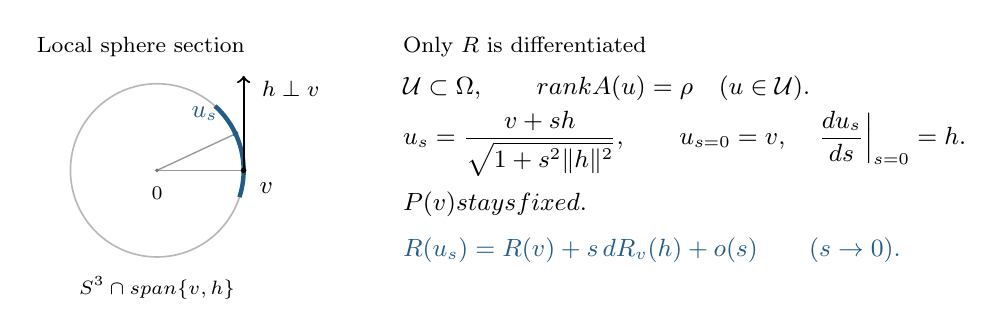
\begin{tikzpicture}[x=1cm,y=1cm,font=\small]
  \definecolor{tangentblue}{RGB}{35,92,135}

  \node[anchor=west,font=\footnotesize] at (0,3.02)
    {Local sphere section};
  \coordinate (O) at (1.65,1.45);
  \coordinate (V) at (2.75,1.45);
  \coordinate (Us) at (2.6469,1.9149); %
  \draw[black!28,line width=0.6pt] (O) circle[radius=1.1];

  \draw[tangentblue,line width=1.6pt]
    (2.6962,1.1101) arc[start angle=-18,end angle=48,radius=1.1];
  \draw[black!40,line width=0.5pt] (O) -- (V);
  \draw[black!40,line width=0.5pt] (O) -- (Us);
  \fill[black!55] (O) circle[radius=0.025];
  \node[anchor=north,font=\scriptsize] at (1.65,1.36) {$0$};

  \draw[->,line width=0.8pt] (V) -- (2.75,2.65);
  \node[anchor=west,font=\footnotesize] at (2.86,2.49) {$h\perp v$};
  \fill (V) circle[radius=0.035];
  \node[anchor=north west] at (2.83,1.42) {$v$};
  \fill[tangentblue] (Us) circle[radius=0.037];
  \node[anchor=south east,text=tangentblue] at (2.54,1.96) {$u_s$};
  \node[anchor=north,font=\scriptsize] at (1.65,0.22)
    {$S^3\cap\operatorname{span}\{v,h\}$};

  \node[anchor=west,font=\footnotesize] at (4.65,3.02)
    {Only $R$ is differentiated};
  \node[anchor=west] at (4.65,2.49)
    {$\mathcal U\subset\Omega,\qquad \operatorname{rank}A(u)=\rho\quad(u\in\mathcal U).$};
  \node[anchor=west] at (4.65,1.79)
    {$\displaystyle u_s=\frac{v+sh}{\sqrt{1+s^2\|h\|^2}},
      \qquad u_{s=0}=v,\quad \left.\frac{du_s}{ds}\right|_{s=0}=h.$};
  \node[anchor=west] at (4.65,1.02)
    {$P(v)\text{ stays fixed.}$};
  \node[anchor=west,text=tangentblue] at (4.65,0.43)
    {$R(u_s)=R(v)+s\,dR_v(h)+o(s)\qquad(s\to0).$};
\end{tikzpicture}
\caption{A schematic local tangent step, for a fixed nonzero $h\in v^\perp$.
The highlighted arc lies in a chosen constant-rank neighborhood $\mathcal U$;
the expansion of $R$ is used only for small $s$ with $u_s\in\mathcal U$.
The pictured section belongs to the parameter sphere, whereas $P(v)$
and $R(u_s)$ act on the separate block spaces $\mathbb R^a$ and
$\mathbb R^c$.}
\label{fig:local-tangent}
\end{figure}


The linear map \(J:v^\perp\to\R^3\) is an isomorphism. Indeed, if
\(Jh=0\), then \(v_0\ne0\) gives
\(h=(h_0/v_0)v\); since \(h\perp v\), this forces \(h=0\).
Both spaces have dimension three.
Consequently the matrix
\[
 F(z,y)=P(v)B(y)dR_v(J^{-1}z),\qquad z,y\in\R^3,
\]
has entries that are bilinear in \(z,y\), since \(B\) and the differential
\(dR_v\) are linear. In fixed orthonormal bases,
each entry \(\ell_{ij}(z,y)\) satisfies
\[
 \ell_{ij}(z,y)^2
 \le \norm{F(z,y)}_{\op}^{2}
 =b(z,y)
 \qquad(z,y\in\R^3).
\]
Lemma~\ref{lem:form} forces every entry to vanish identically.
Equation~\eqref{eq:tangent-identity} would therefore make \(b\)
identically zero, contradicting \(b(e_1,e_1)=1\).
This excludes the hypothetical finite pencil and completes the proof.
\end{proof}
